\chapter{Webová aplikace}
V této kapitole budou představeny jednotlivé aplikace, jejich funkce a způsob integrace s vyvinutými nástroji \texttt{framesss} a \texttt{desssign}.

Webová aplikace, vyvinutá za podpory poskytnuté Ministerstvem průmyslu a obchodu ČR v rámci programu OP PIK, Aplikace (Výzva IX), č. projektu CZ.01.1.02/0.0/0.0/21\_374/0026789, \textit{Vývoj komplexního softwaru pro optimalizaci návrhu a posouzení střešních a stropních konstrukcí}, zahrnuje dvě hlavní aplikace: STŘECHA a STROP. Tato kapitola popisuje jednotlivé aplikace, jejich funkce a integraci s vyvinutými knihovnami \texttt{framesss} a \texttt{desssign}.

Aplikace slouží pro předběžné ověření dimenzí konstrukčních prvků s využitím řešení a výrobků společnosti Wienerberger.

V rámci diplomové práce bylo vyvinuto nové uživatelské prostředí, které bylo zatím implementováno jen do aplikace STŘECHA. Aplikaci STROP tento přechod čeká v nejbližší době.

\section{Aplikace STŘECHA}
Aplikace STŘECHA je určena pro předběžný návrh konstrukčních prvků krovu se střešními krytinami a skladbami Tondach. V rámci této diplomové práce došlo k výraznému zlepšení grafického uživatelského rozhraní a interakce s uživatelem.

\subsection{Původní verze aplikace}
Původní verze aplikace STŘECHA poskytovala základní nástroje pro posouzení krovů. Uživatel procházel jednotlivými kroky, od zadání geometrie objektu, přes zadání lokality pro výpočet klimatických zatížení, zvolení krytiny, skladby střešního pláště, až po definování průřezů a materiálů jednotlivých prvků. Následně byla takto zadaná konstrukce posouzena na několik předem definovaných kombinací zatížení, které uživatel nemohl upravit.

Původní uživatelské prostředí bylo tvořeno několika velkými statickými formuláři, který byly sice přehledné, ale velmi dlouhé. Uživatelé zároveň neměli žádnou vizuální kontrolu nad tím, co zadávají, což mohlo vést k chybám při zadávání dat. Výsledky byly prezentovány ve formě textového výstupu, ve velmi stručné formě, což omezovalo možnosti interaktivní zpětné vazby.

\begin{figure}[H]
    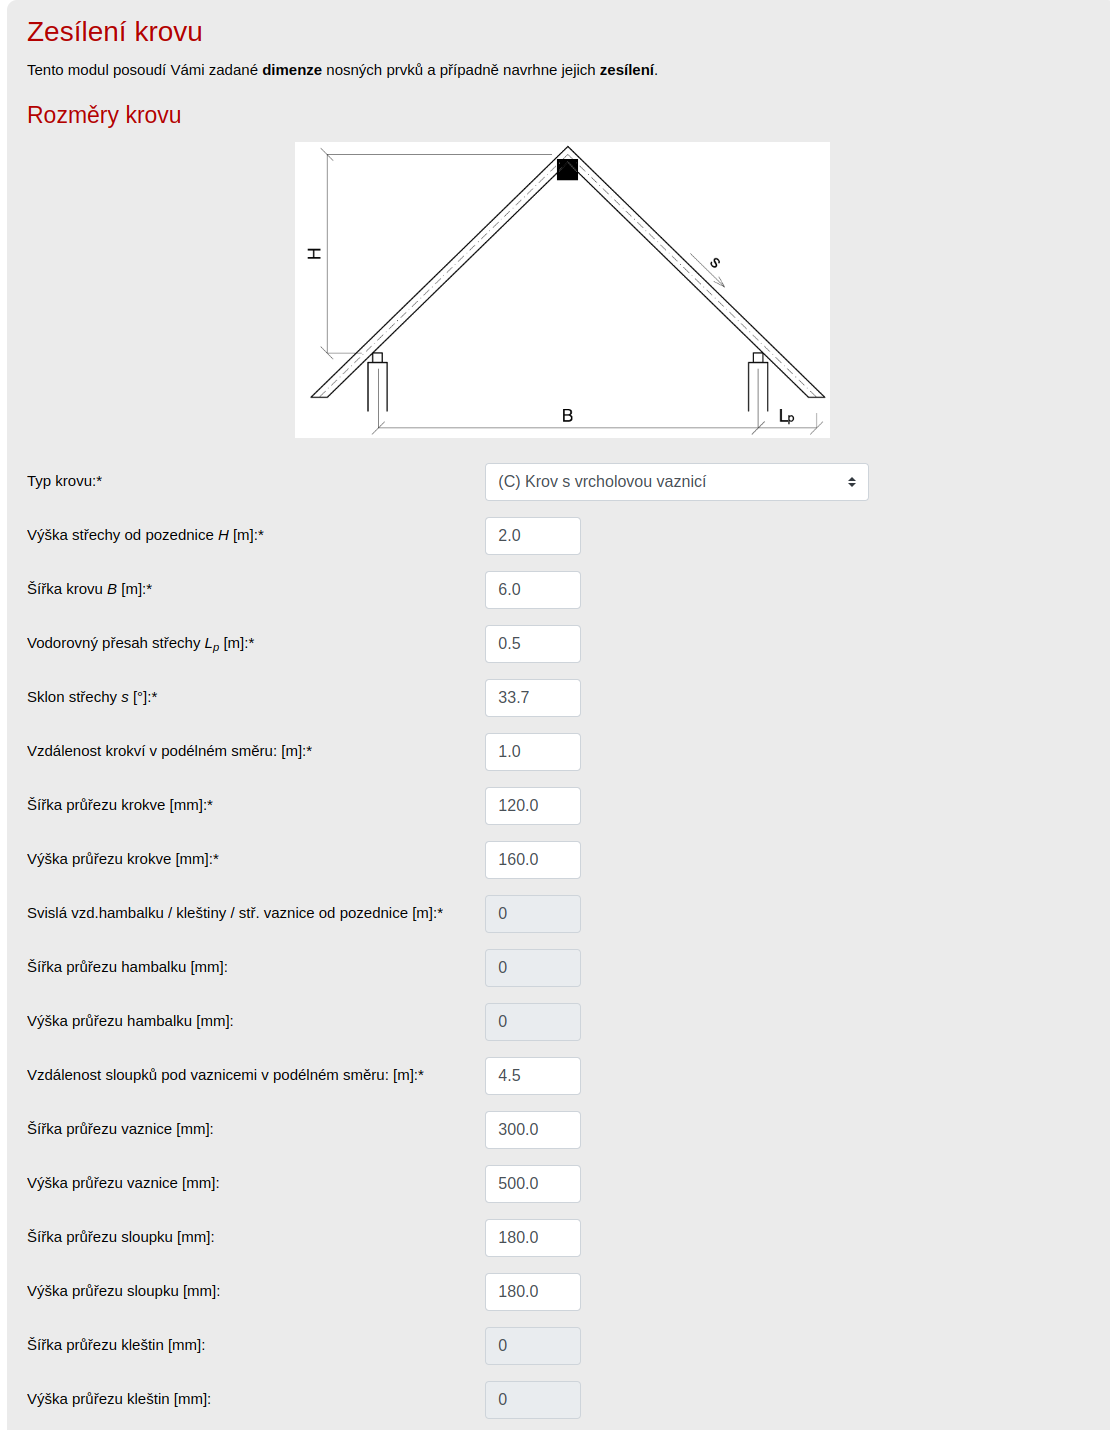
\includegraphics{assets/figures/wbapp/strecha_old-0-0.png}
    \caption{STŘECHA -- Modul pro finální posouzení 1/2}
    \label{fig:roof_old_1}
\end{figure}

\begin{figure}[H]
    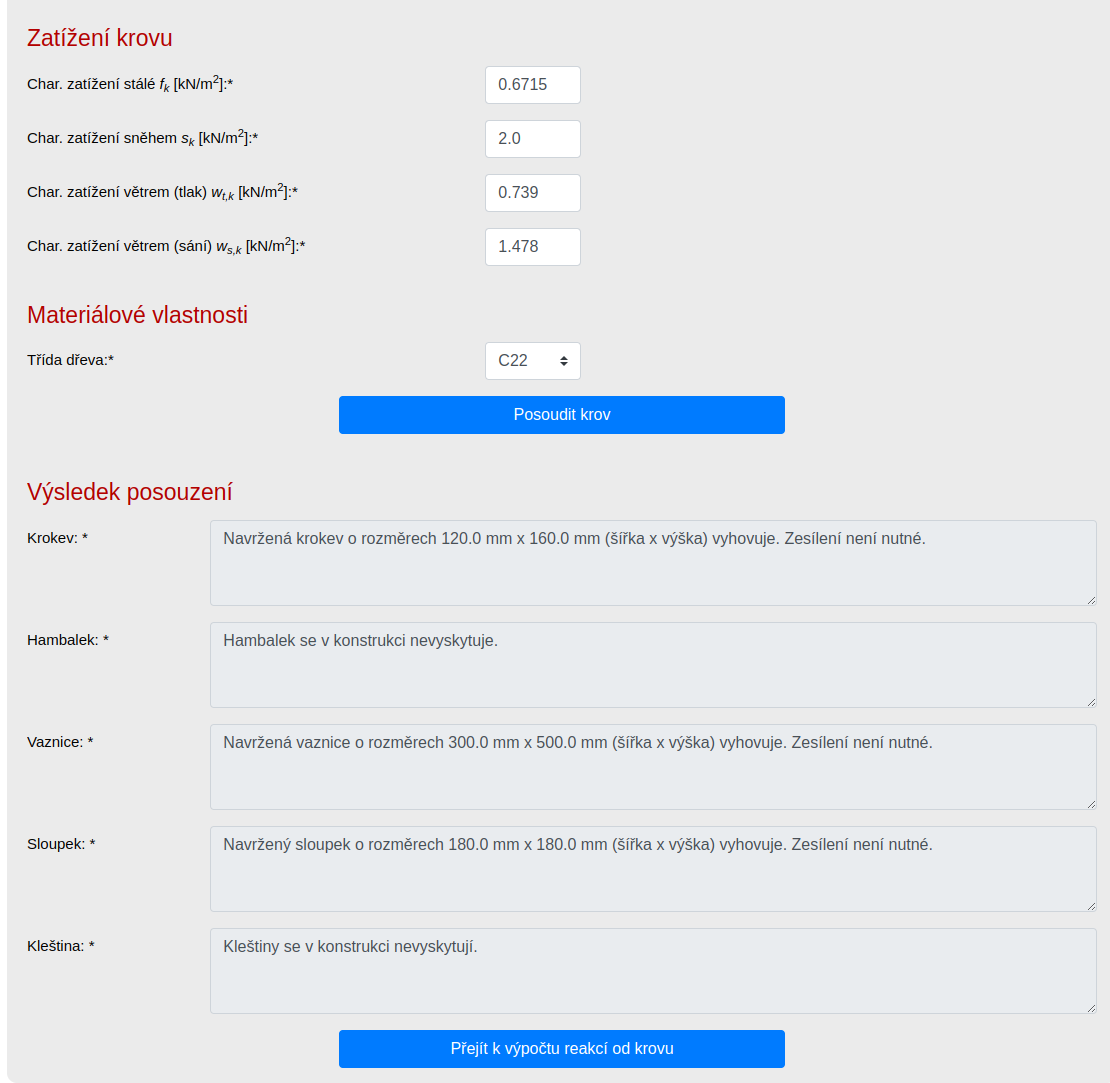
\includegraphics{assets/figures/wbapp/strecha_old-0-1.png}
    \caption{STŘECHA -- Modul pro finální posouzení 2/2}
    \label{fig:roof_old_2}
\end{figure}


\subsection{Nová verze}
Nová verze aplikace STŘECHA přináší výrazné zlepšení v uživatelském rozhraní a interaktivitě. Používá moderní technologie pro dynamickou vizualizaci a umožňuje uživatelům interaktivně modelovat střešní konstrukce.

\subsubsection*{Funkčnost}
Nová verze aplikace STŘECHA umožňuje uživatelům projít několika kroky k vygenerování statického schématu se zatíženími a zatěžovacími stavy, podobně jako tomu bylo v původní verzi. Nově však může měnit geometrii, přidávat a ubírat zatížení, definovat zatěžovací stavy, kombinovat je do kombinací a zobrazovat si výsledky pro jednotlivé stavy zvlášť.

Pro všechny tyto funkce aplikace využívá knihovny \texttt{framesss} a \texttt{desssign}, které byly představeny v předchozích kapitolách.

\subsubsection*{Uživatelské prostředí}
Nové uživatelské prostředí aplikace STŘECHA nabízí intuitivní a interaktivní rozhraní, které uživatelům umožňuje snadno zadávat data a mít nad nimi vizuální kontrolu.

V hlavní části obrazovky se nachází vizualizace modelu střechy, kde jsou zobrazeny uzly, prvky a aplikovaná zatížení. Uživatel může interaktivně přidávat uzly, prvky a zatížení pomocí ovládacích prvků v dolní části obrazovky. Tento přístup zajišťuje, že uživatelé mají přehled o všech zadaných datech a mohou je snadno upravovat a kontrolovat.

Uživatel může v prostředí aplikace:
\begin{itemize}
    \item generovat střešní konstrukci z předdefinovaných typů střešních konstrukcí,
    \item přidávat, editovat a mazat entity,
    \item vypočítat vnitřní síly,
    \item posoudit konstrukci.
\end{itemize}

\begin{figure}[H]
    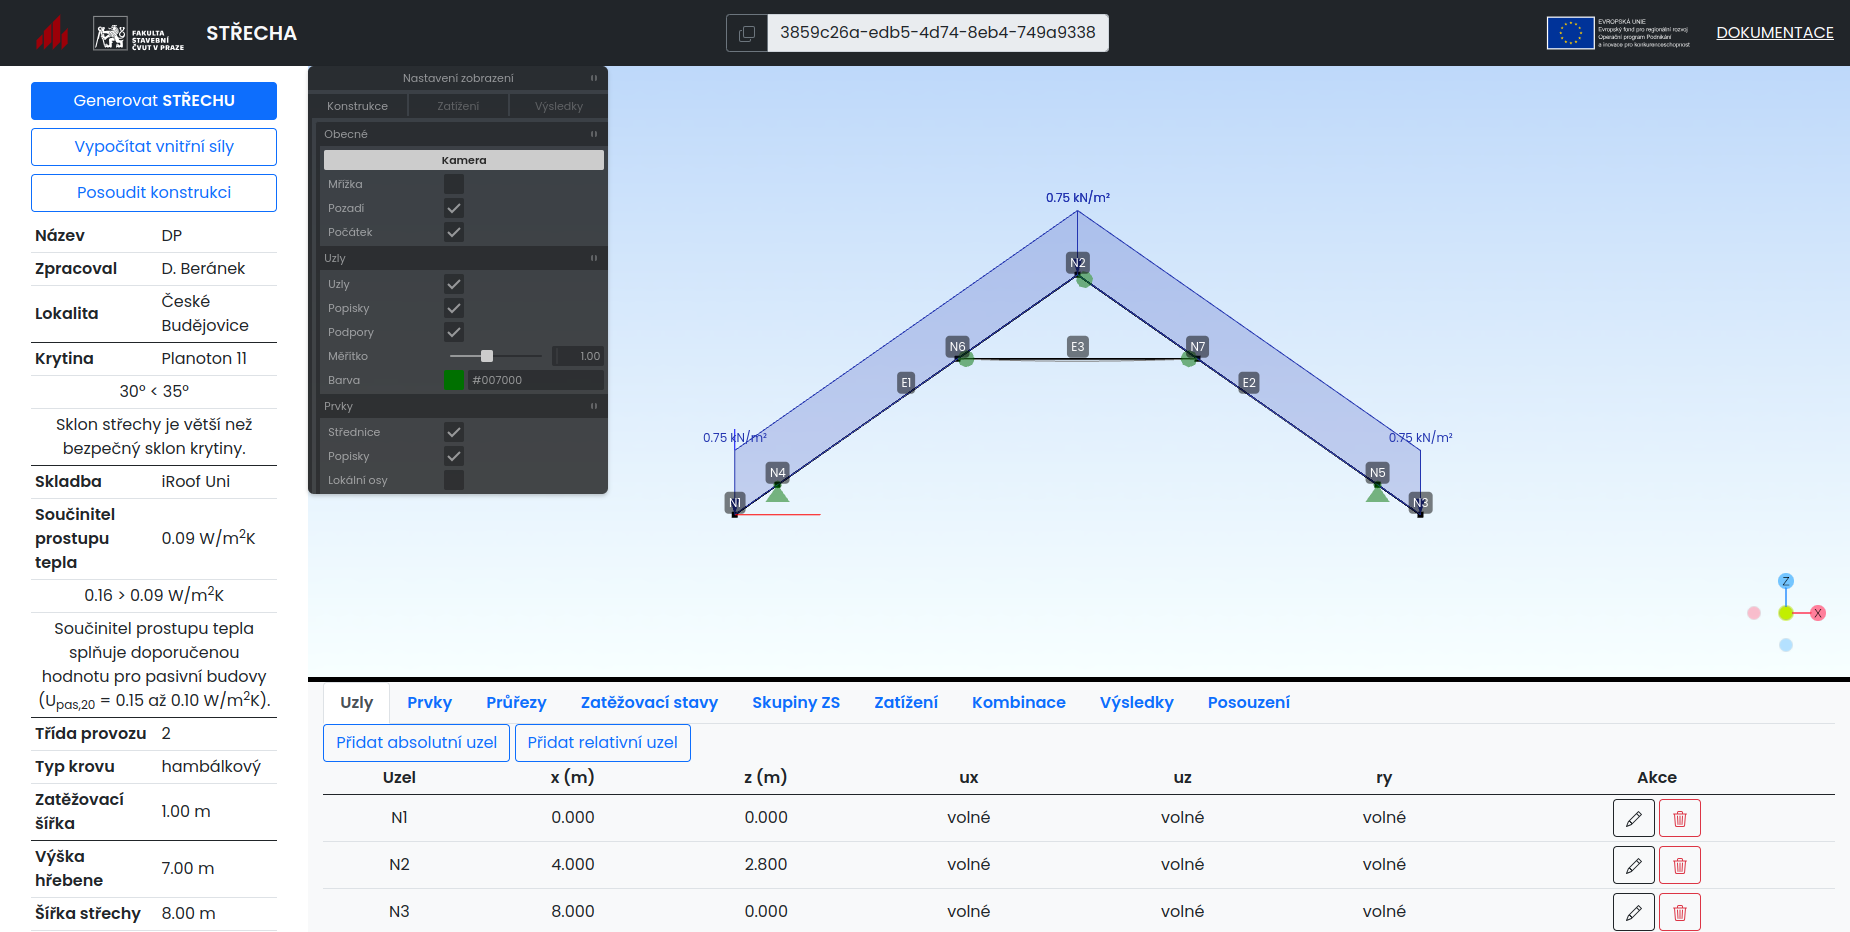
\includegraphics{assets/figures/wbapp/strecha_new.png}
    \caption{STŘECHA -- Nové uživatelské prostředí}
    \label{fig:roof_new}
\end{figure}

Na obrázku \autoref{fig:roof_new} je rozvržení nového uživatelského prostředí, na levé straně obrazovky se nachází panel s informacemi o projektu, jako je název, zpracovatel, lokalita, krytina, sklon střechy, skladba, součinitel prostupu tepla, typ krovu a další. V hlavní části obrazovky se nachází vizualizace statického modelu, kde jsou zobrazeny uzly, prvky a aplikovaná zatížení. Uživatel může interaktivně přidávat, měnit a mazat uzly, prvky, zatížení a veškeré další objekty pomocí ovládacích prvků v záložkách v dolní části obrazovky. Tento přístup zajišťuje, že uživatelé mají přehled o všech zadaných datech a mohou je snadno upravovat a kontrolovat.

\subsubsection*{Spodní panel}
V dolní části obrazovky se nachází karty s ovládacími prvky a přehlednými tabulkami, které zobrazují veškeré informace o modelované konstrukci. Tyto karty zahrnují:
\begin{itemize}
    \item \textbf{Uzly}: Seznam všech uzlů v modelu s jejich souřadnicemi a definicí podepření v jednotlivých směrech.
    \item \textbf{Prvky}: Seznam všech prvků, pro každý prvek se zde zobrazují jeho výchozí a koncový uzel, relativně zadané uzly, koncové klouby, délka a průřez.
    \item \textbf{Průřezy}: Seznam všech prvků s definicí materiálu a základních geometrických veličin.
    \item \textbf{Zatěžovací stavy}: Seznam všech zatěžovacích stavů, jejich typ, kategorie, třída trvání zatížení a odpovídající součinitele podle ČSN EN 1990.
    \item \textbf{Skupiny ZS}: Skupiny zatěžovacích stavů, ze kterých se generují kombinace.
    \item \textbf{Zatížení}: Seznam spojitých a bodových zatížení na prvcích a v uzlech. Na této kartě lze přepínat mezi zatěžovacími stavy. Zatížení pro aktivní zatěžovací stav se zobrazuje ve vizualizaci.
    \item \textbf{Kombinace}: Seznam všech kombinací, jejich mezní stav, typ a kombinační klíč.
    \item \textbf{Výsledky}: Seznam vnitřních sil ve všech průřezech, kde se může vyskytovat extrém vnitřních sil. Na této kartě lze přepínat mezi zatěžovacími stavy a kombinacemi zatížení. Pro aktivní výběr se vykreslují výsledky v modelu.
    \item \textbf{Posouzení}: Přehled využití jednotlivých prutů.
\end{itemize}

Na každé kartě je tlačítko pro přidání nové entity do modelu. Zároveň lze každou entitu, kromě zatížení vlastní tíhou, vymazat nebo upravit.

\begin{figure}[H]
    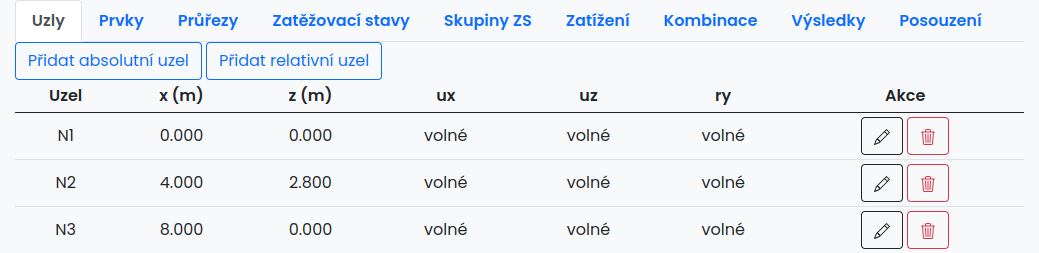
\includegraphics{assets/figures/wbapp/nodes_tab.png}
    \caption{STŘECHA -- Záložka s uzly}
    \label{fig:nodes}
\end{figure}

\begin{figure}[H]
    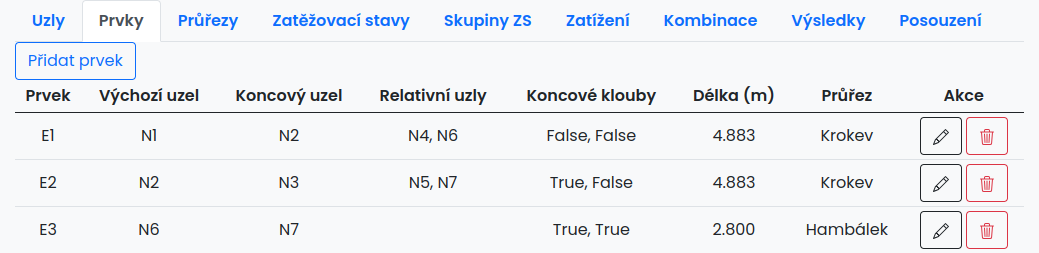
\includegraphics{assets/figures/wbapp/members_tab.png}
    \caption{STŘECHA -- Záložka s prvky}
    \label{fig:members}
\end{figure}

\begin{figure}[H]
    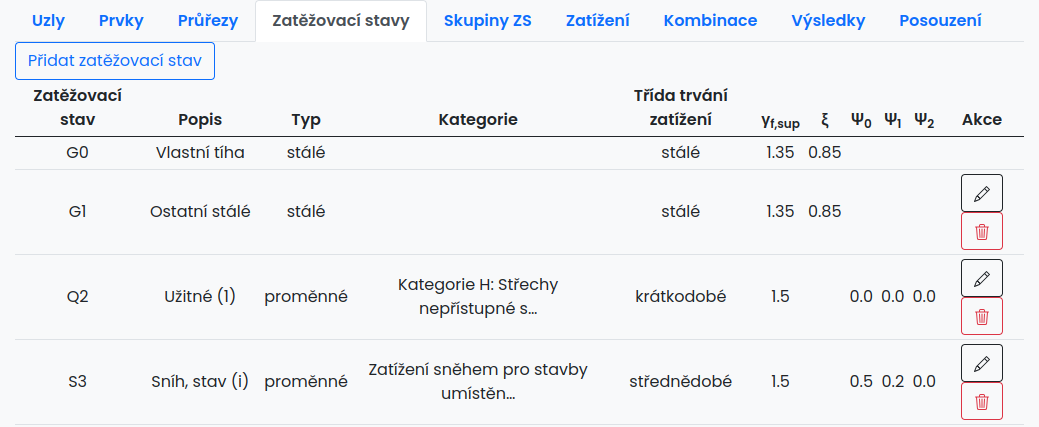
\includegraphics{assets/figures/wbapp/load_cases_tab.png}
    \caption{STŘECHA -- Záložka se zatěžovacími stavy}
    \label{fig:load_cases}
\end{figure}

\begin{figure}[H]
    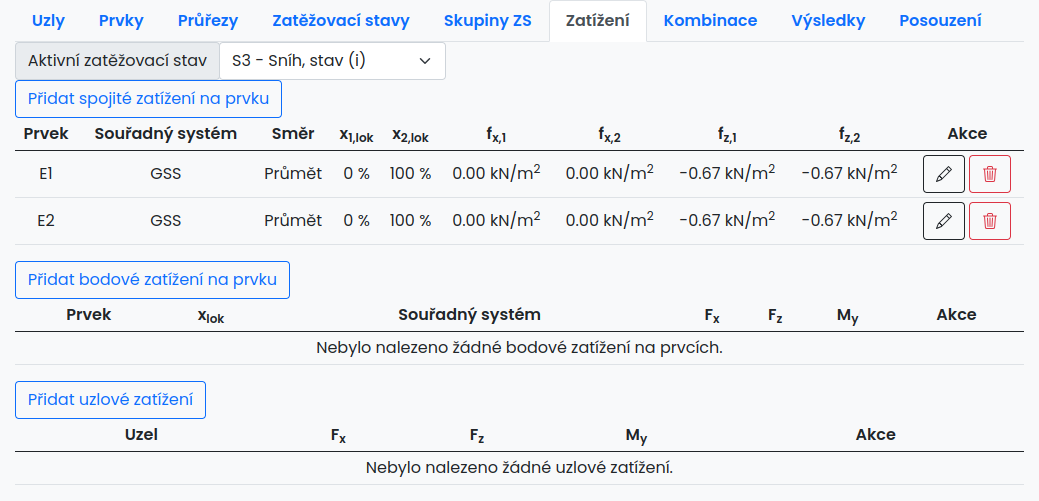
\includegraphics{assets/figures/wbapp/loads_tab.png}
    \caption{STŘECHA -- Záložka se zatížením}
    \label{fig:loads}
\end{figure}

\begin{figure}[H]
    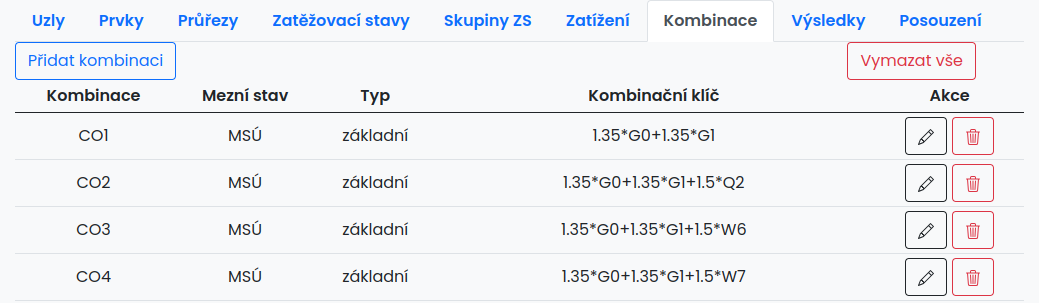
\includegraphics{assets/figures/wbapp/combos_tab.png}
    \caption{STŘECHA -- Záložka s kombinacemi zatížení}
    \label{fig:combos_tab}
\end{figure}

\subsubsection*{Editace entit}
Téměř každou entitu lze editovat. Po kliknutí na tlačítko \textbf{Přidat} nebo \textbf{Editovat} se zobrazí okno umožňující zadání potřebných údajů.
\begin{figure}[H]
    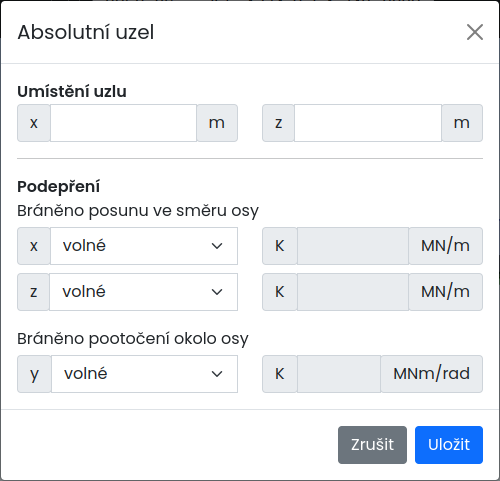
\includegraphics[width=7.5cm]{assets/figures/wbapp/add_node_modal.png}
    \caption{STŘECHA -- Okno pro přidání nového uzlu}
    \label{fig:add_node}
\end{figure}

\begin{figure}[H]
    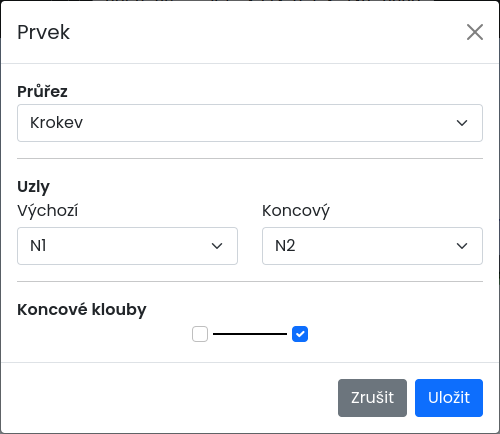
\includegraphics[width=7.5cm]{assets/figures/wbapp/add_member_modal.png}
    \caption{STŘECHA -- Okno pro přidání nového prvku}
    \label{fig:add_member}
\end{figure}

\begin{figure}[H]
    \includegraphics[width=7.5cm]{assets/figures/wbapp/add_load_Case_modal.png}
    \caption{STŘECHA -- Okno pro přidání nového zatěžovacího stavu}
    \label{fig:add_load_case}
\end{figure}

